\section{A szimuláció eredményei}
\begin{frame}
	\frametitle{A szimuláció eredményei}
	\begin{block}{Adatok összevetése}
		A már rendelkezésünkre álló bemeneti paraméterekre\cite{archetti2016cooperation} elvégeztünk 100-100 szimulációt, minden egyes diffúziós távolságra 1-től 5-ig.
	\end{block}

	\begin{block}{Paraméterek}
		\begin{multicols}{2}
			\begin{itemize}
				\item populáció mérete: 1000
				\item defektálók: 5\%
				\item generációk száma: 15
				\item kooperálók költsége: 0.01
				\item osztódás: nincs
			\end{itemize}
			\begin{itemize}
				\item $s = 2$
				\item $k = 1$
				\item $d = \frac{1}{2}D$
				\item $z = 20$
			\end{itemize}	
		\end{multicols}
	\end{block}
\end{frame}

\begin{frame}
	\frametitle{Összehasonlítás}
	\begin{figure}[h]
		\centering
		\begin{tabular}{cc}
			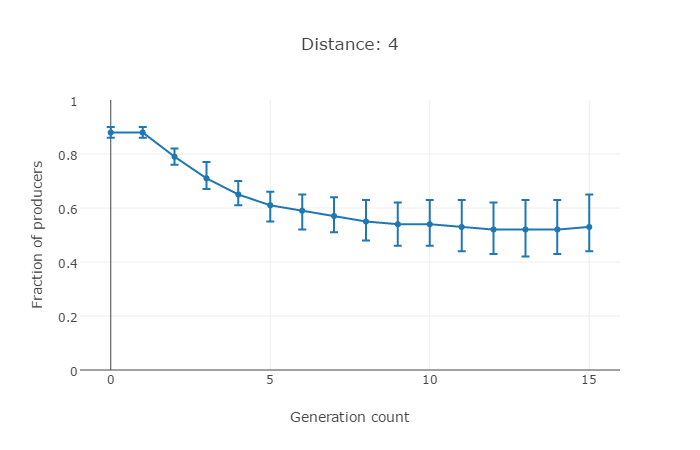
\includegraphics[width=0.4\linewidth]{images/dist4}
			&
			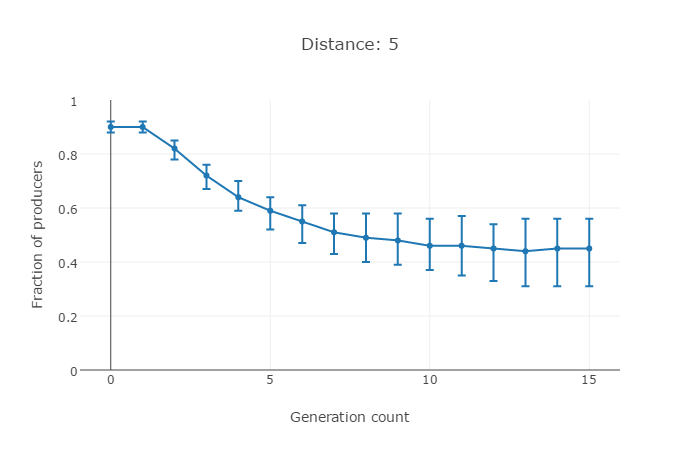
\includegraphics[width=0.4\linewidth]{images/dist5}
			\\
			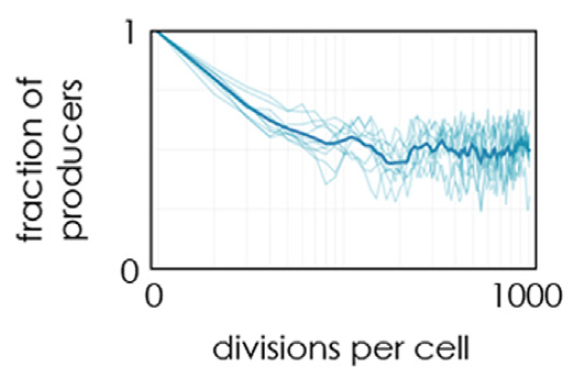
\includegraphics[width=0.4\linewidth]{images/arc_dist4}
			&
			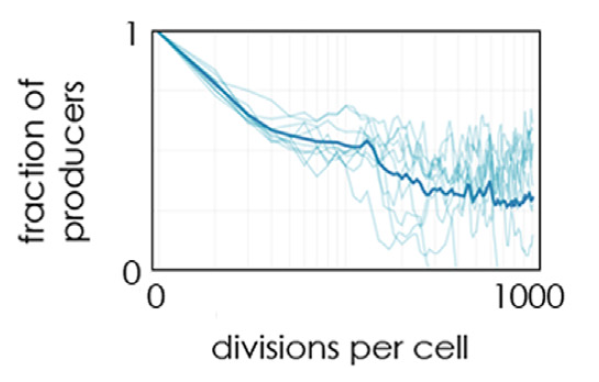
\includegraphics[width=0.4\linewidth]{images/arc_dist5}
			\\
		\end{tabular}
		\caption{Szimulációs eredmények a fenti paraméterekre és azok párjai a \cite{archetti2016cooperation} cikkből}
		\label{fig:DistChange}
	\end{figure}
\end{frame}

\subsection{A költség és nyereség hatása}
\begin{frame}
	\frametitle{A költség és nyereség hatása}
	\begin{block}{}
		Minél többe kerül a termelés annál jobban megéri élősködni. Az esetek többségében a defektálás a legkifizetődőbb, de alacsony költségek mellett fenntartható egy bizonyos egyensúly is a két fél között.
	\end{block}
	
	\begin{figure}[h]
		\centering
		\begin{tabular}{cc}
			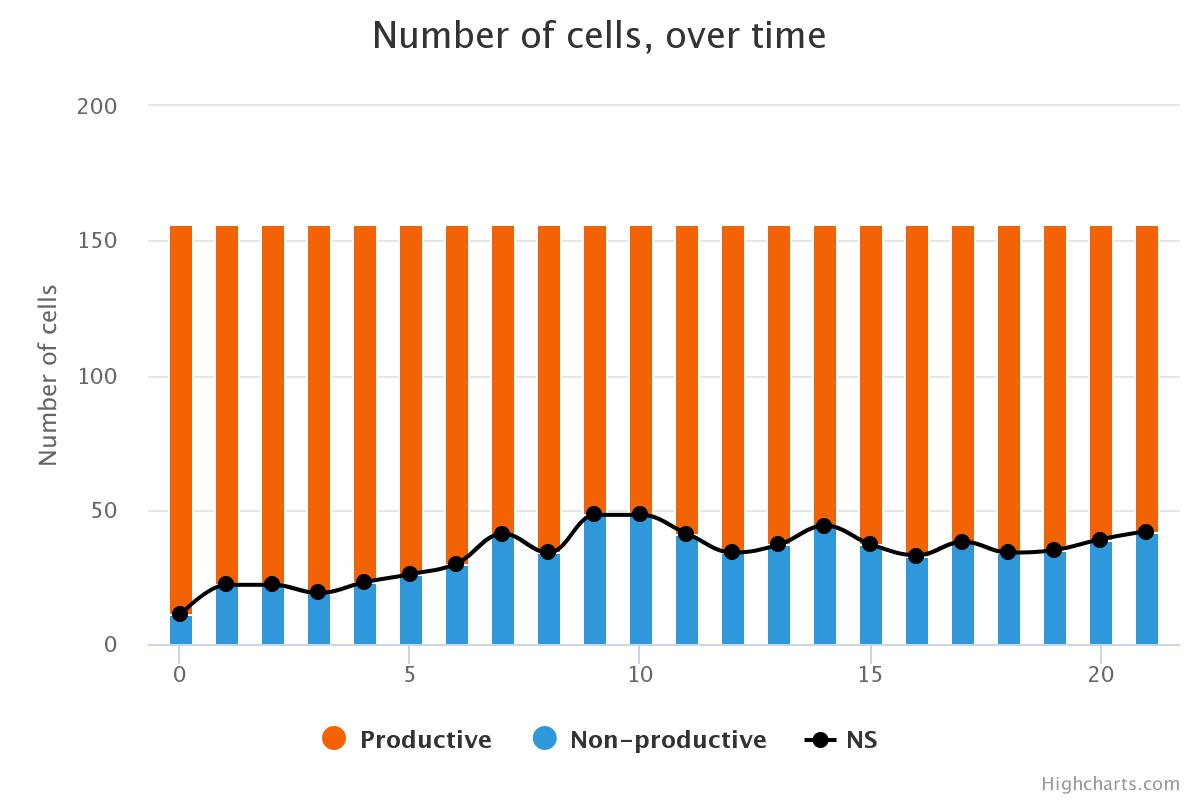
\includegraphics[width=0.35\linewidth]{images/chart001.jpeg}
			&
			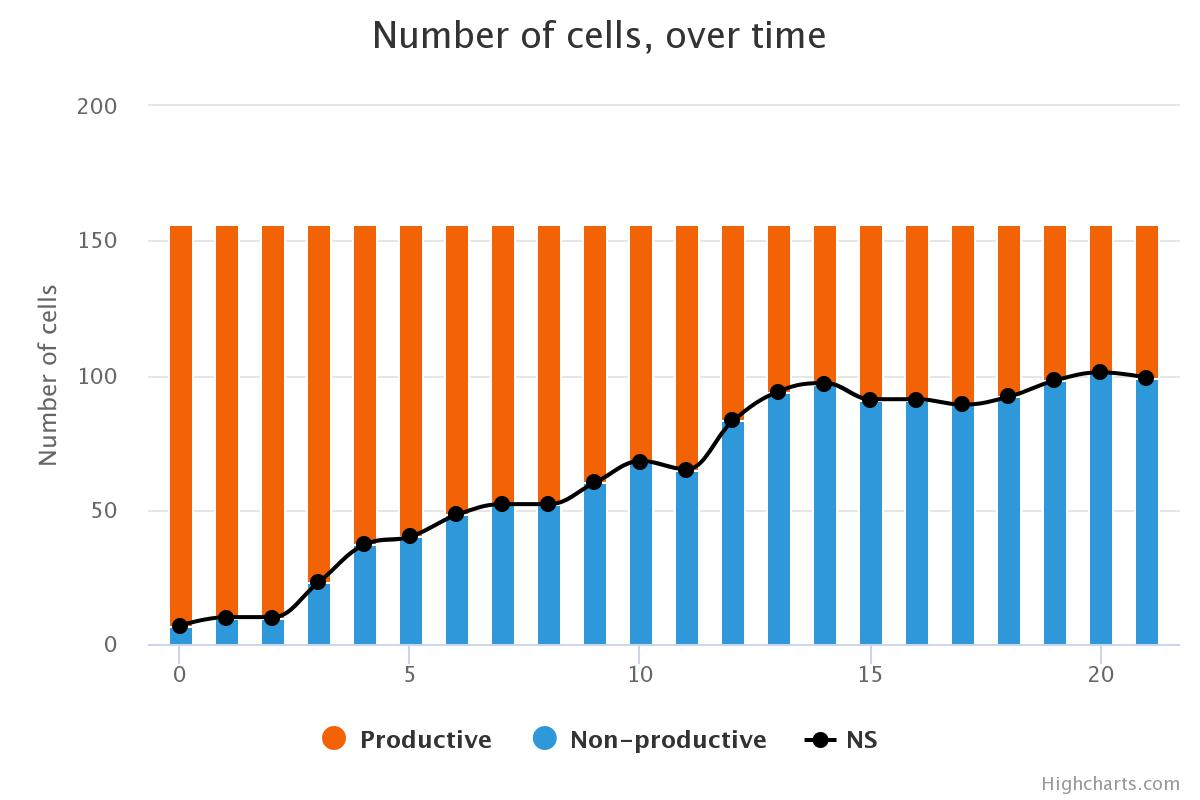
\includegraphics[width=0.35\linewidth]{images/chart01.jpeg}
		\end{tabular}
		\begin{tabular}{cl}  
			\begin{tabular}{c}
				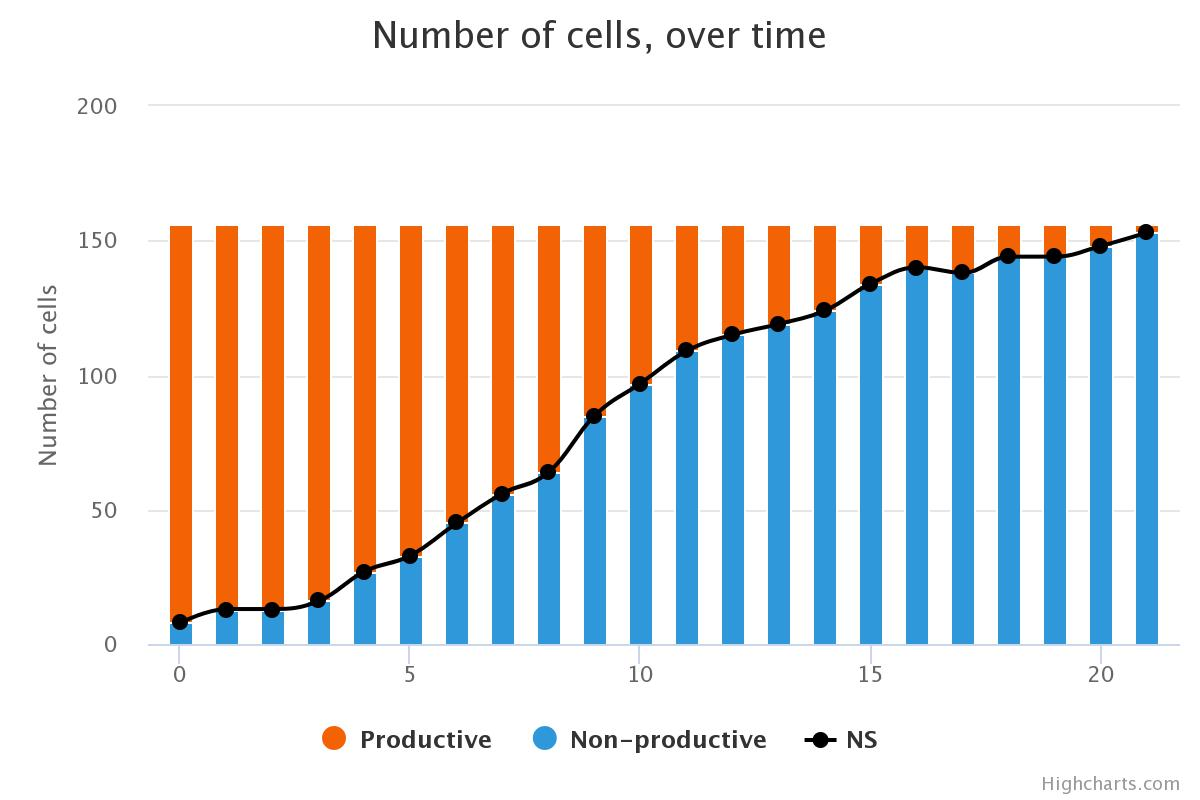
\includegraphics[width=0.35\linewidth]{images/chart08.jpeg}
			\end{tabular}
			& 
			\begin{tabular}{l}
				\parbox{0.35\linewidth}{
					A játék végkimenetele mikor a költségek rendre 0.01, 0.1 és 0.8
				}
			\end{tabular}  \\
		\end{tabular}
		\label{fig:CoopCostChange}
	\end{figure}
\end{frame}

\subsection{Diffúziós távolság hatása}
\begin{frame}
	\frametitle{Diffúziós távolság hatása}
	\begin{itemize}
		\item a diffúziós távolság növelésével valósághűbb adatokat kaphatunk
		\item a távolság növekedésével a defektáló sejtek könnyebben terjednek
		\item ezt a paramétert a hasnyálmirigyrák esetén megállapították\cite{archetti2015heterogeneity}
	\item az esetek túlnyomó részében ez az érték 5-10-től 30-60-ig terjedhet\cite{archetti2016cooperation}
	\end{itemize}
	
	\begin{figure}[h]
		\centering
		\begin{tabular}{cc}
			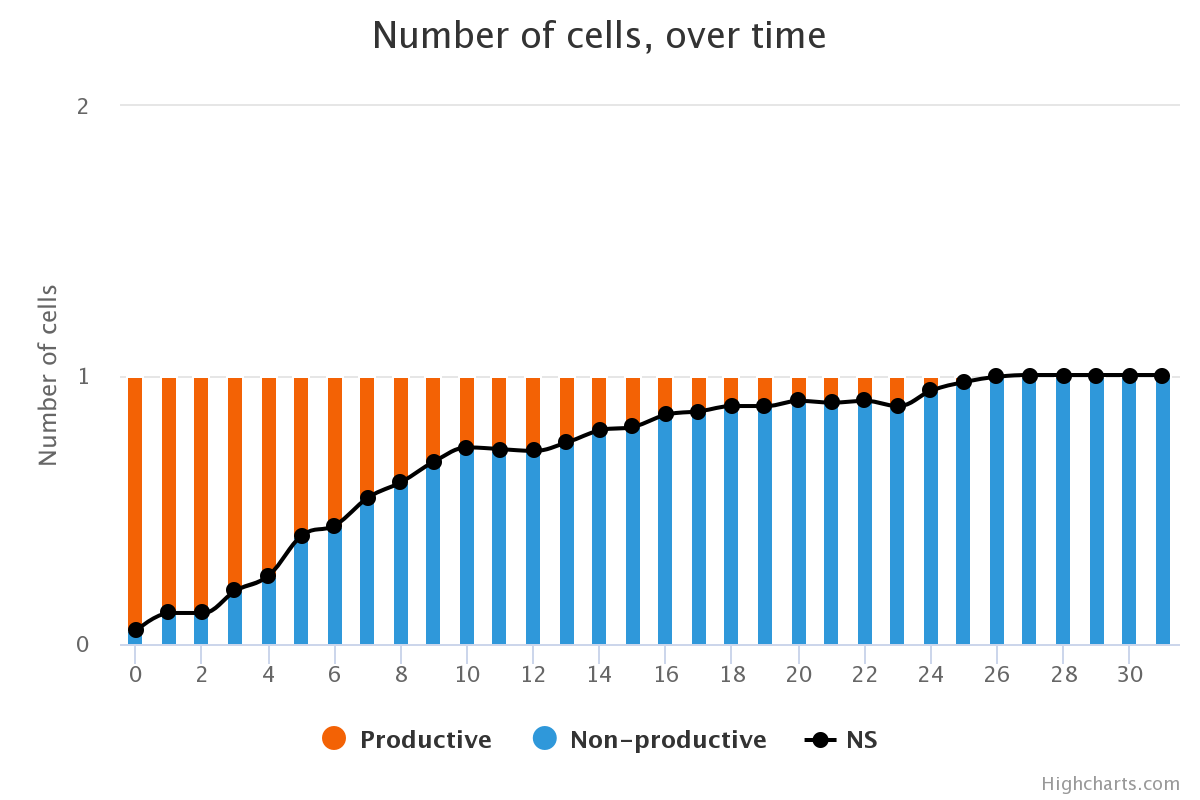
\includegraphics[width=0.4\linewidth]{images/diffdist2}
			&
			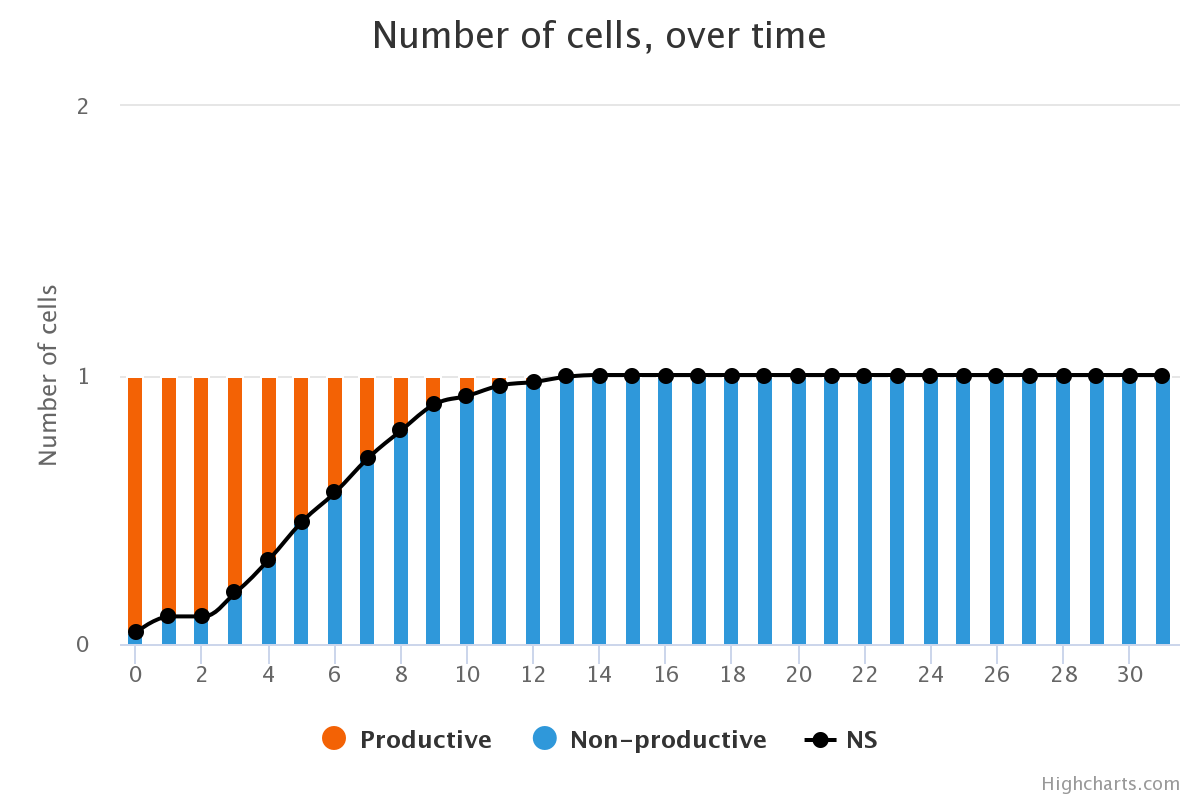
\includegraphics[width=0.4\linewidth]{images/diffdist5}
		\end{tabular}
		\caption{A játék végkimenetele két diffúziós távolságra. A paraméterek: 160 sejt, 5\% defektáló, 0.3 költség, távolság: 2 illetve 5}
		\label{fig:DiffDist}
	\end{figure}
\end{frame}

\subsection{Osztódásra képes populációk}
\begin{frame}
	\frametitle{Osztódásra képes populációk}
	\begin{itemize}
		\item eddigi a populáció mérete állandó volt és egy adott modellt követett
		\item a valóságban a defektáló sejtek nem csak területileg terjednek el
		\item számosságban is túlnövik a kooperálókat
	\end{itemize}
	
	\begin{columns}
		\column{0.5\textwidth}
			\begin{figure}[ht]
				\centering
				\begin{tabular}{c}
					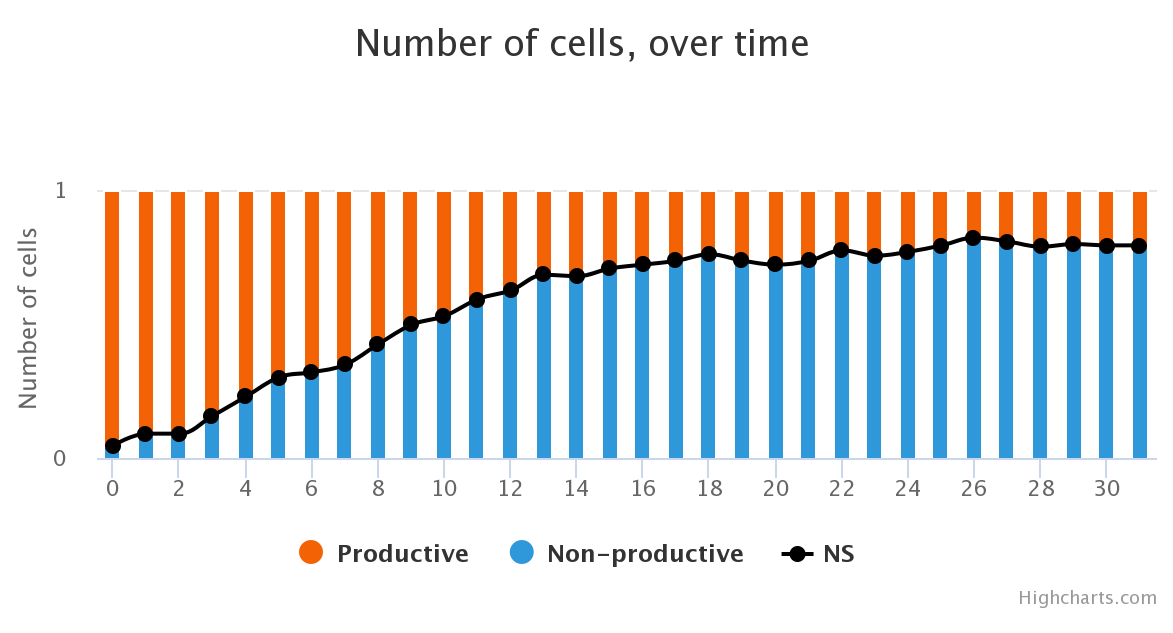
\includegraphics[width=0.9\textwidth]{images/nemosztodik}
					\\
					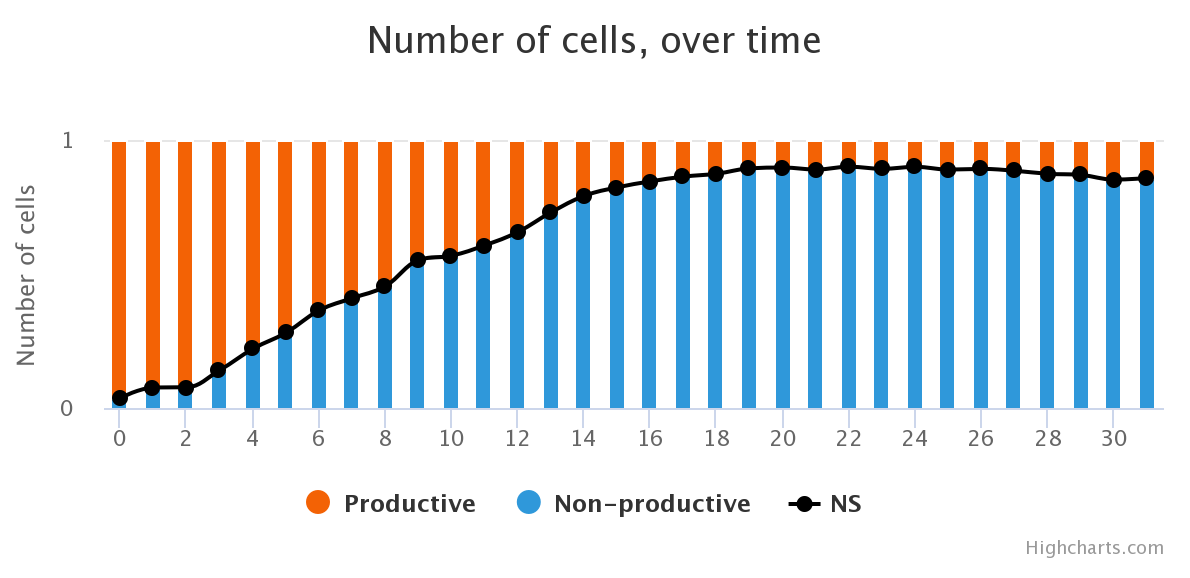
\includegraphics[width=0.9\textwidth]{images/osztodik}
				\end{tabular}
				\caption{Az első esetben a sejtek nem osztódtak míg a másodikban igen}				\label{fig:Divide}
			\end{figure}
		\column{0.5\textwidth}
			\begin{block}{}
				Az osztódás során létrejött új sejtek képesek felgyorsítani a defektálók terjedését, de ezen területen még további kísérletek szükségesek, hogy pontosabb képet kapjunk arról, hogy ez mennyire befolyásolja a játék végkimenetelét.
			\end{block}
	\end{columns}
\end{frame}

\begin{frame}
	\frametitle{Osztódással vagy anélkül?}
	\begin{table}
		\caption{Osztódás nélküli modell}
		\label{table:nemOsztodik}
		\adjustbox{max height=\dimexpr\textheight-5.5cm\relax, max width=\textwidth}{
			\begin{tabular}{ | l | l | l | l | l | l | l | l | l | l | l | l | }
				\hline
				\multirow{3}{*}{D = 2}
				& Generáció & 1 & 2 & 3 & 4 & 5 & 6 & 7 & 8 & 9 & 10 \\ \cline{2-12}
				& CoopPerc & 0.91 & 0.91 & 0.85 & 0.81 & 0.77 & 0.75 & 0.73 & 0.71 & 0.69 & 0.68 \\ \cline{2-12}
				& stdev & 0.01 & 0.01 & 0.02 & 0.03 & 0.03 & 0.03 & 0.05 & 0.05 & 0.05 & 0.06 \\ \hline
				\multirow{3}{*}{D = 3}
				& Generáció & 1 & 2 & 3 & 4 & 5 & 6 & 7 & 8 & 9 & 10 \\ \cline{2-12}
				& CoopPerc & 0.9 & 0.9 & 0.83 & 0.77 & 0.72 & 0.68 & 0.66 & 0.64 & 0.62 & 0.6 \\ \cline{2-12}
				& stdev & 0.02 & 0.02 & 0.03 & 0.04 & 0.04 & 0.05 & 0.04 & 0.05 & 0.05 & 0.04 \\ \hline
			\end{tabular}
		}
	\end{table}
	
	\begin{table}
		\caption{Osztódást használó modell}
		\label{table:osztodik}
		\adjustbox{max height=\dimexpr\textheight-5.5cm\relax, max width=\textwidth}{
			\begin{tabular}{ | l | l | l | l | l | l | l | l | l | l | l | l | }
				\hline
				\multirow{3}{*}{D = 2}
				& Generáció & 1 & 2 & 3 & 4 & 5 & 6 & 7 & 8 & 9 & 10 \\ \cline{2-12}
				& CoopPerc & 0.87 & 0.87 & 0.79 & 0.74 & 0.7 & 0.67 & 0.64 & 0.61 & 0.59 & 0.57 \\ \cline{2-12}
				& stdev & 0.02 & 0.02 & 0.03 & 0.04 & 0.05 & 0.06 & 0.07 & 0.05 & 0.07 & 0.07 \\ \hline
				\multirow{3}{*}{D = 3}
				& Generáció & 1 & 2 & 3 & 4 & 5 & 6 & 7 & 8 & 9 & 10 \\ \cline{2-12}
				& CoopPerc & 0.89 & 0.9 & 0.82 & 0.75 & 0.7 & 0.66 & 0.62 & 0.59 & 0.56 & 0.54 \\ \cline{2-12}
				& stdev & 0.03 & 0.04 & 0.05 & 0.06 & 0.08 & 0.08 & 0.08 & 0.09 & 0.09 & 0.09 \\ \hline
			\end{tabular}
		}
	\end{table}
\end{frame}
